\section{Introduction}


\label{sec:intro}

Modern AI demands fast inference. Yet standard language model decoding generates single tokens sequentially, failing to leverage the massive parallel computation available on modern hardware. Speculative decoding \citep{leviathan2023, chen2023} (SD) is a technique introduced to alleviate this problem. 
Instead of slow, autoregressive sampling from a desired ``target model," it uses a fast ``draft model'' to predict the next few tokens that would be generated by the target model and 
then ``verifies'' these tokens in one \textit{parallel} forward pass of the target model. This verification is done according to an algorithm that guarantees the resulting tokens are drawn from the distribution of the target model.
In each verification, the target model decides both how many speculated tokens to accept, \textit{and} samples an additional \textit{bonus token} that follows all of the accepted tokens.
%This exploits the key fact that verifying many tokens \textit{in parallel} is much faster than generating them \textit{sequentially}.
Though speculative decoding is effective, it is \textit{itself} limited by a \textit{sequential} dependence: verification must complete before the next speculation can begin. We ask: 
\begin{center}
\textit{Can we eliminate the sequential dependence between drafting and verification?}
\end{center}

We introduce \textit{speculative speculative decoding} (SSD), a unifying framework for methods that aim to parallelize drafting and verification.
While in SD the draft model \textit{waits} for the verification to complete before beginning to speculate the next round,
in SSD the draft model \textit{predicts} what verification outcomes are most likely, and prepares (i.e., pre-speculates) for all of them \textit{in parallel} to the verification taking place.
If any of these prepared outcomes occurs, the draft model can \textit{immediately} send the pre-speculated tokens to the verifier, thereby avoiding all draft overhead. 
Like ordinary speculative decoding, SSD is lossless. Unlike ordinary speculative decoding, in SSD the draft model is located on distinct hardware from the target. 

\begin{figure}[ht]
\centering
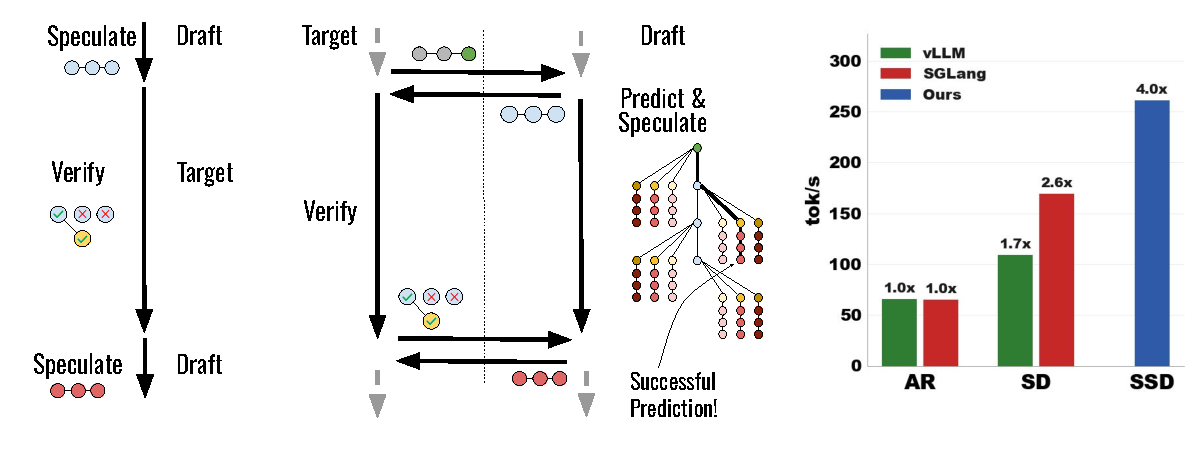
\includegraphics[width=\textwidth]{figures/ssd_fig1.pdf}

\caption{
    (Left) Ordinary speculative decoding (SD) requires the verifier to wait idly for the draft to speculate. 
    (Center) In our algorithm, speculation runs on a separate device (1$\times$H100) in parallel with verification; the draft precomputes speculations for many possible verification outcomes and returns the speculated tokens immediately if one occurs.
    (Right) \textit{End-to-end performance} of SSD, SD, and autoregressive (AR) decoding averaged over four datasets spanning math, code and chat, for Llama-3.1-70B on TP=4 H100s, batch size 1, greedy decoding, Llama-3.2-1B draft model.
}
\label{fig:fig1}
\end{figure}

There are three main challenges in optimizing SSD algorithms.
First, the draft model must correctly anticipate the verification outcome, which includes not just how many speculated tokens were accepted, but \textit{which} bonus token was sampled. 
Second, we identify a subtle trade-off between the acceptance rate of the speculator and how well it is able to predict verification outcomes, which must be navigated carefully to maximize speedups.
Third, any SSD algorithm must have a fallback strategy to handle failed attempts at predicting verification outcomes correctly.
At large batch sizes and temperatures, these failures happen increasingly often and naïvely speculating just-in-time negates the benefits of asynchrony.

% In resolving these challenges, we present \Sys, an optimized SSD algorithm. 
% \textbf{\Sys achieves decoding speedups of up to 2x compared to optimized speculative decoding baselines, and up to 5x that of standard autoregressive generation on a range of datasets and model families (Figure \ref{fig:e2e}).}
% It incorporates targeted optimizations for each challenge:

We present \Sys, an optimized SSD algorithm that incorporates targeted optimizations for each challenge:

\begin{itemize}
    \item In Section~\ref{sec:cache_topology}, we frame the 
    problem of predicting verification outcomes in terms of constrained optimization, and introduce a technique that uses the most likely draft logits to predict the bonus token, doing so with up to 90\% accuracy.
    \item In Section~\ref{sec:cache_sampling}, we identify a tension between accurately predicting verification outcomes and generating high-quality speculations, and develop a sampling algorithm that allows balancing the two. Appendix~\ref{app:saguaro_construction} gives a construction where this new sampling scheme necessarily yields end-to-end speedups.
    \item In Section~\ref{sec:cache_misses}, we examine various strategies to handle failed predictions, demonstrating that the optimal fallback strategy varies with batch size.
    Adopting this, \Sys outperforms SD 20\% even at larger batch sizes, despite doing more compute per batch element by decoding many possible outcomes simultaneously.
\end{itemize}
% \Needspace{3\baselineskip}

\textbf{Altogether, \Sys achieves up to 2x speedup over optimized speculative decoding and up to 5x over autoregressive generation (Figure~\ref{fig:e2e}), while strictly improving the throughput-latency Pareto frontier across a range of batch sizes.}